% Technical report: dengue in Peru, an Apache Spark analysis.
% Build with `latexmk` from this folder (see .latexmkrc): the PDF and auxiliary files go to build/,
% which is not versioned. Each section lives in sections/; figures are read from ../figures/.
\documentclass[11pt,a4paper]{article}

% Language and fonts. es-noshorthands keeps < and > free for TikZ; es-tabla names tables "Tabla".
\usepackage[T1]{fontenc}
\usepackage[spanish,es-noshorthands,es-tabla,es-nodecimaldot]{babel}
\usepackage{amsmath}
\usepackage{lmodern}                 % typewriter font for code
\usepackage{newtxtext,newtxmath}     % Times for text and math
\usepackage{microtype}
\usepackage{csquotes}

% Page layout
\usepackage[a4paper,margin=2cm]{geometry}
\usepackage{enumitem}
\setlist{itemsep=1pt,topsep=3pt}

% Figures, tables and diagrams
\usepackage{graphicx}
\graphicspath{{../figures/}}
\usepackage{booktabs}
\usepackage{tabularx}
\usepackage{array}
\usepackage{caption}
\captionsetup{font=small,labelfont=bf,skip=4pt}
\setlength{\textfloatsep}{10pt plus 2pt minus 2pt}
\setlength{\floatsep}{8pt plus 2pt minus 2pt}
\setlength{\intextsep}{8pt plus 2pt minus 2pt}
\usepackage{subcaption}
\usepackage{tikz}
\usetikzlibrary{arrows.meta,positioning}

% Code and execution plans
\usepackage{xcolor}
\usepackage{listings}
\lstset{basicstyle=\ttfamily\footnotesize, columns=fullflexible, keepspaces=true, frame=single,
        framerule=0.4pt, rulecolor=\color{black!30}, breaklines=true, xleftmargin=3pt, xrightmargin=3pt,
        aboveskip=6pt, belowskip=6pt}
\lstdefinestyle{plan}{basicstyle=\ttfamily\fontsize{6.6}{7.6}\selectfont, breaklines=false}

% References in IEEE style
\usepackage[style=ieee,backend=biber]{biblatex}
\addbibresource{references.bib}
\renewcommand*{\bibfont}{\small}

\usepackage[hidelinks]{hyperref}

\newcommand{\code}[1]{\texttt{#1}}

\title{Dengue en el Perú: análisis de datos con Apache Spark\\[4pt]\large Informe técnico}
\author{Raymond Negron\\[2pt]\small Ciencia de Datos Escalable · Maestría en Ciencia de Datos}
\date{Noviembre de 2026}

\begin{document}

\maketitle

\begin{abstract}
Este informe analiza el dengue en el Perú entre 2000 y 2025 con Apache Spark, integrando cinco fuentes de datos
abiertos oficiales: casos notificados, población, emergencias hídricas, establecimientos de salud y estaciones
meteorológicas. Con la DataFrame API y Spark SQL se responden seis preguntas: los brotes son cada vez más grandes,
la mayor incidencia está en la costa norte, y los distritos en emergencia por lluvias o con menos horas de agua
tuvieron más casos. Además, se siguen consultas reales desde el logical plan hasta los stages, tasks y shuffles,
para explicar cómo Spark convierte las operaciones en una ejecución distribuida.
\end{abstract}

\section{Introducción y descripción del problema}
\label{sec:introduction}

El dengue es una enfermedad viral transmitida por el mosquito \emph{Aedes aegypti}, que se reproduce en agua
acumulada. En el Perú es un problema de salud pública creciente: el sistema de vigilancia registra más de un
millón de casos entre 2000 y 2025, y las epidemias de 2023 y 2024 fueron las más grandes del periodo.

Este proyecto usa datos abiertos oficiales del Estado peruano para responder seis preguntas sobre el dengue:
cómo evolucionó, dónde y en quiénes tiene mayor incidencia, y cómo se relaciona con la cobertura de
establecimientos de salud, las emergencias hídricas y la lluvia. Todo el procesamiento se hace con las
Structured APIs de Apache Spark, la DataFrame API y Spark SQL \cite{zaharia2016,armbrust2015}.

Además de los resultados, el proyecto responde la pregunta central del curso: \emph{¿cómo transforma Spark
las operaciones de análisis en una ejecución distribuida?} Para ello se siguen consultas reales del análisis
desde el logical plan hasta los stages y tasks que se ejecutan, y se mide el shuffle que generan.

\section{Datasets y fuentes}
\label{sec:datasets}

Se usan cinco fuentes oficiales y públicas (Tabla~\ref{tab:datasets}): cuatro de la Plataforma Nacional de
Datos Abiertos \cite{datosabiertos} y una de la API de interoperabilidad del SENAMHI. La llave común es el
\code{ubigeo}, el código de 6 dígitos de cada distrito (2 del departamento, 2 de la provincia y 2 del distrito).

\begin{table}[htbp]
\centering
\caption{Datasets del proyecto. \emph{Filas}: tamaño de cada tabla después de la preparación con Spark.}
\label{tab:datasets}
\small
\begin{tabularx}{\textwidth}{@{}>{\raggedright\arraybackslash}p{4.1cm} >{\raggedright\arraybackslash}p{2.2cm} X r@{}}
\toprule
Dataset (publicador) & Cobertura & Contenido y uso & Filas \\
\midrule
Vigilancia de dengue (CDC Perú – MINSA) \cite{ds-dengue} & 2000–2025 &
  Un caso notificado por fila: distrito, semana epidemiológica, edad, sexo y diagnóstico (CIE-10).
  Tabla principal. & 1,065,274 \\
Población identificada con DNI (RENIEC) \cite{ds-reniec} & dic. 2022–2025 &
  Población por distrito, sexo y edad. Denominador de las tasas. & 75,636 \\
Distritos en emergencia hídrica (SUNASS) \cite{ds-sunass} & 2017, 2023, 2024 &
  Un distrito por decreto: tipo de emergencia (lluvias o déficit hídrico) y horas de agua al día. & 9,538 \\
Establecimientos de salud, RENIPRESS (SUSALUD) \cite{ds-renipress} & corte al 30-09-2026 &
  Establecimientos activos por distrito y nivel de atención. & 26,972 \\
Estaciones meteorológicas (SENAMHI) \cite{senamhi-api} & 2022–2025 &
  Lluvia, temperatura y humedad diarias de 9 estaciones de la costa norte y la selva. & 12,827 \\
\bottomrule
\end{tabularx}
\end{table}

La población por distrito solo existe desde 2022, así que todas las tasas usan 2022–2025. Es la población con
DNI según el domicilio declarado, no la población censal. Los datos del SENAMHI no tienen control de calidad y
algunas estaciones tienen días sin registro.

Para que el análisis sea reproducible, \code{data/catalog.yaml} registra la URL y el hash SHA-256 de cada
archivo, y un script los descarga y verifica. Los datos no se versionan: solo el CSV de dengue pesa 118~MB.

\section{Preguntas de análisis}
\label{sec:questions}

Las preguntas (Tabla~\ref{tab:questions}) van de la descripción del problema a su relación con la salud, el
agua y el clima. Todas, salvo la primera, integran al menos dos datasets.

\begin{table}[htbp]
\centering
\caption{Preguntas de análisis y datasets que usa cada una.}
\label{tab:questions}
\small
\begin{tabularx}{\textwidth}{@{}l X >{\raggedright\arraybackslash}p{3.8cm}@{}}
\toprule
 & Pregunta & Datasets \\
\midrule
Q1 & ¿Cómo evolucionó el dengue entre 2000 y 2025 y qué años fueron epidémicos? & dengue \\
Q2 & ¿Qué distritos tuvieron la mayor incidencia (casos por 100,000 habitantes) en 2022–2025? & dengue, población \\
Q3 & ¿Qué grupos de edad y qué sexo tienen la mayor incidencia? & dengue, población \\
Q4 & ¿La proporción de casos con signos de alarma o graves se relaciona con la cobertura de establecimientos de
     salud? & dengue, establecimientos, población \\
Q5 & ¿Los distritos en emergencia hídrica tuvieron mayor incidencia? ¿Influye la continuidad del servicio de
     agua? & dengue, población, emergencias \\
Q6 & ¿Cuántas semanas después de la lluvia aumentan los casos, y es distinto en la costa y en la selva? &
     dengue, estaciones \\
\bottomrule
\end{tabularx}
\end{table}

\section{Arquitectura de la solución}
\label{sec:architecture}

La solución es un pipeline de tres notebooks de PySpark sobre archivos locales (Figura~\ref{fig:architecture}).
Un script descarga las fuentes y verifica su hash; el notebook 01 las lee con Spark, las limpia y las guarda como
tablas Parquet; los notebooks 02 y 03 leen esas tablas para responder las preguntas y analizar la ejecución.

\begin{figure}[htbp]
\centering
\begin{tikzpicture}[
    box/.style={draw=black!50, rounded corners=2pt, align=center, font=\footnotesize, text width=33mm,
                minimum height=13mm, fill=#1},
    box/.default=white,
    spark/.style={box=blue!10, draw=blue!60},
    arrow/.style={-{Stealth[length=2mm]}, thick, black!55}]
  % Row 1: from the sources to the prepared tables
  \node[box=black!5] (src)  at (0, 0)     {\textbf{Fuentes}\\datosabiertos.gob.pe (CSV)\\API SENAMHI (JSON)};
  \node[box=black!5] (dl)   at (4.3, 0)   {\code{download\_data.py}\\\code{catalog.yaml}\\(URL, SHA-256)};
  \node[box]         (raw)  at (8.6, 0)   {\code{data/raw/}\\datos originales};
  \node[spark]       (prep) at (12.9, 0)  {\textbf{01 · Preparación}\\esquema explícito,\\limpieza};
  % Row 2: analysis on the Parquet tables
  \node[box]         (proc)  at (12.9, -2.7) {\code{data/processed/}\\5 tablas Parquet};
  \node[spark, minimum height=9mm] (an)    at (8.6, -2.05) {\textbf{02 · Análisis}\\DataFrame API};
  \node[spark, minimum height=9mm] (plans) at (8.6, -3.35) {\textbf{03 · Ejecución}\\Spark SQL, \code{explain}};
  \node[box=black!5] (out)   at (4.3, -2.7)  {\textbf{Resultados}\\figuras, planes\\e informe};
  \draw[arrow] (src) -- (dl);
  \draw[arrow] (dl) -- (raw);
  \draw[arrow] (raw) -- (prep);
  \draw[arrow] (prep) -- (proc);
  \draw[arrow] (proc) -- (an);
  \draw[arrow] (proc) -- (plans);
  \draw[arrow] (an) -- (out);
  \draw[arrow] (plans) -- (out);
  \node[font=\footnotesize, anchor=west] at (-1.65, -2.7)
       {\tikz\filldraw[fill=blue!10, draw=blue!60] (0,0) rectangle (3mm,3mm);~Apache Spark};
\end{tikzpicture}
\caption{Arquitectura de la solución. Los pasos en azul se ejecutan con Apache Spark 4.2.1.}
\label{fig:architecture}
\end{figure}

Spark corre en local mode: una sola JVM donde el driver planifica el trabajo y 12 executor threads, uno por
core, ejecutan las tasks. El mismo código correría sin cambios en un cluster. Las principales decisiones de
diseño son:
\begin{itemize}
  \item \textbf{Parquet como formato intermedio.} Es columnar, así que Spark lee solo las columnas que necesita
        (column pruning). Los casos se guardan particionados por \code{year}, una carpeta por año, y una consulta
        puede saltar los años que no usa (partition pruning).
  \item \textbf{Esquemas explícitos.} Las fuentes se leen sin \code{inferSchema}: se evita una pasada extra por
        los archivos y el \code{ubigeo} se mantiene como texto, sin perder los ceros iniciales.
  \item \textbf{Spark como herramienta principal.} No se usa Pandas; matplotlib solo dibuja resultados que Spark
        ya agregó (unas decenas de filas).
\end{itemize}

El entorno usa Spark 4.2.1 (PySpark), Python 3.11 y Java 25. El código y las instrucciones de ejecución están en
el repositorio del proyecto \cite{repo}.

\section{Procesamiento con Apache Spark}
\label{sec:processing}

\subsection{Lectura y preparación}

Cada fuente necesitó un tratamiento distinto (Tabla~\ref{tab:preparation}). En todas se renombraron las columnas
al inglés y el resultado se escribió en Parquet.

\begin{table}[htbp]
\centering
\caption{Transformaciones principales de la preparación (notebook 01).}
\label{tab:preparation}
\small
\begin{tabularx}{\textwidth}{@{}l X@{}}
\toprule
Fuente & Transformaciones \\
\midrule
Dengue & Edad normalizada a años (venía en años, meses o días); gravedad a partir del código CIE-10; semana
         epidemiológica convertida en la fecha de su domingo (\code{week\_start}) para alinearla con el clima. \\
RENIEC & Un archivo por año: el año se toma del nombre del archivo con la columna oculta
         \code{\_metadata.file\_path}. Se excluye a los peruanos en el extranjero y se suma la población por
         distrito, sexo y etapa de vida. \\
SUNASS & Archivo en Latin-1; tipo de emergencia (lluvias, déficit hídrico u otra) derivado de la descripción del
         decreto; marca de prórroga. \\
RENIPRESS & Separador \code{;} y direcciones con saltos de línea: sin \code{multiLine=True} y
         \code{escape='"'} se perdían filas. Solo establecimientos activos. \\
SENAMHI & JSON anidado: dos \code{explode} lo llevan a una fila por estación, día y variable, y un \code{pivot}
         devuelve una columna por variable. \\
\bottomrule
\end{tabularx}
\end{table}

\subsection{Análisis}

Las seis preguntas se resuelven con la DataFrame API (notebook 02). Se usan transformaciones (\code{select},
\code{filter}, \code{withColumn}, \code{when}, \code{fillna}, \code{pivot}, \code{unpivot}), agregaciones
(\code{groupBy} y \code{agg} con \code{count}, \code{sum}, \code{avg}, \code{min}, \code{max} y \code{corr}, y
\code{orderBy}) y window functions (\code{lag}, \code{lead}, \code{rowsBetween}, \code{row\_number},
\code{dense\_rank}, \code{ntile}). Cada join se eligió según lo que la pregunta necesita conservar
(Tabla~\ref{tab:joins}).

\begin{table}[htbp]
\centering
\caption{Tipos de join usados y su justificación.}
\label{tab:joins}
\small
\begin{tabularx}{\textwidth}{@{}l l X@{}}
\toprule
Join & Dónde & Justificación \\
\midrule
\code{left} & Q2, Q4, Q5, Q6 & La tabla que guía la consulta conserva todas sus filas: distritos sin
  establecimientos (Q4), distritos con 0 casos (Q5), semanas sin casos (Q6). \\
\code{inner} & Q3 & Casos y población cubren la misma grilla completa (2 sexos × 5 etapas de vida): no se
  pierde nada. \\
\code{left\_anti} & Q2 & Verificación: ningún distrito-año con casos queda sin población (resultado: 0). \\
\code{left\_semi} & Q5 & Filtra los casos de distritos con decreto sin duplicarlos. Un distrito aparece una vez
  por decreto y por prórroga: un inner join devuelve 1,539,044 filas en lugar de 352,213. \\
\code{cross} & Q6 & Cada estación con un calendario de 209 semanas, para que \code{lead} avance semanas y no
  filas cuando faltan datos. \\
\bottomrule
\end{tabularx}
\end{table}

\subsection{DataFrame API y Spark SQL}

La consulta de Q2 (los cinco distritos con mayor incidencia por año) se escribió también en Spark SQL, sobre
temporary views. Las dos versiones devuelven el mismo resultado (\code{exceptAll} en ambas direcciones da 0
filas) y, desde el optimized logical plan, el mismo plan (Sección~\ref{sec:plans}). Por ejemplo, el ranking:

\begin{lstlisting}
# DataFrame API
by_year = Window.partitionBy("year").orderBy(F.desc(F.col("cases") / F.col("population")))
F.dense_rank().over(by_year).alias("rank")
-- Spark SQL
DENSE_RANK() OVER (PARTITION BY year ORDER BY cases / population DESC) AS rank
\end{lstlisting}

\section{Resultados y discusión}
\label{sec:results}

\paragraph{Q1 · Evolución y años epidémicos.} El dengue avanza por brotes cada vez más grandes: pasó de unos
5 mil casos en 2000 a un récord de 272 mil en 2024 (Figura~\ref{fig:q1}). Un año es epidémico cuando supera el
doble del promedio de los cinco años anteriores, calculado con una window (\code{rowsBetween(-5, -1)}). Hubo
seis años epidémicos: 2001, 2008, 2011, 2017, 2023 y 2024. Los de 2001, 2017 y 2023 fueron brotes de la costa
norte, liderados por Piura; los de 2008 y 2011, de la Amazonía, liderados por Loreto. Juntos, 2023 y 2024 suman
la mitad de todos los casos desde 2000.

\begin{figure}[!htbp]
\centering
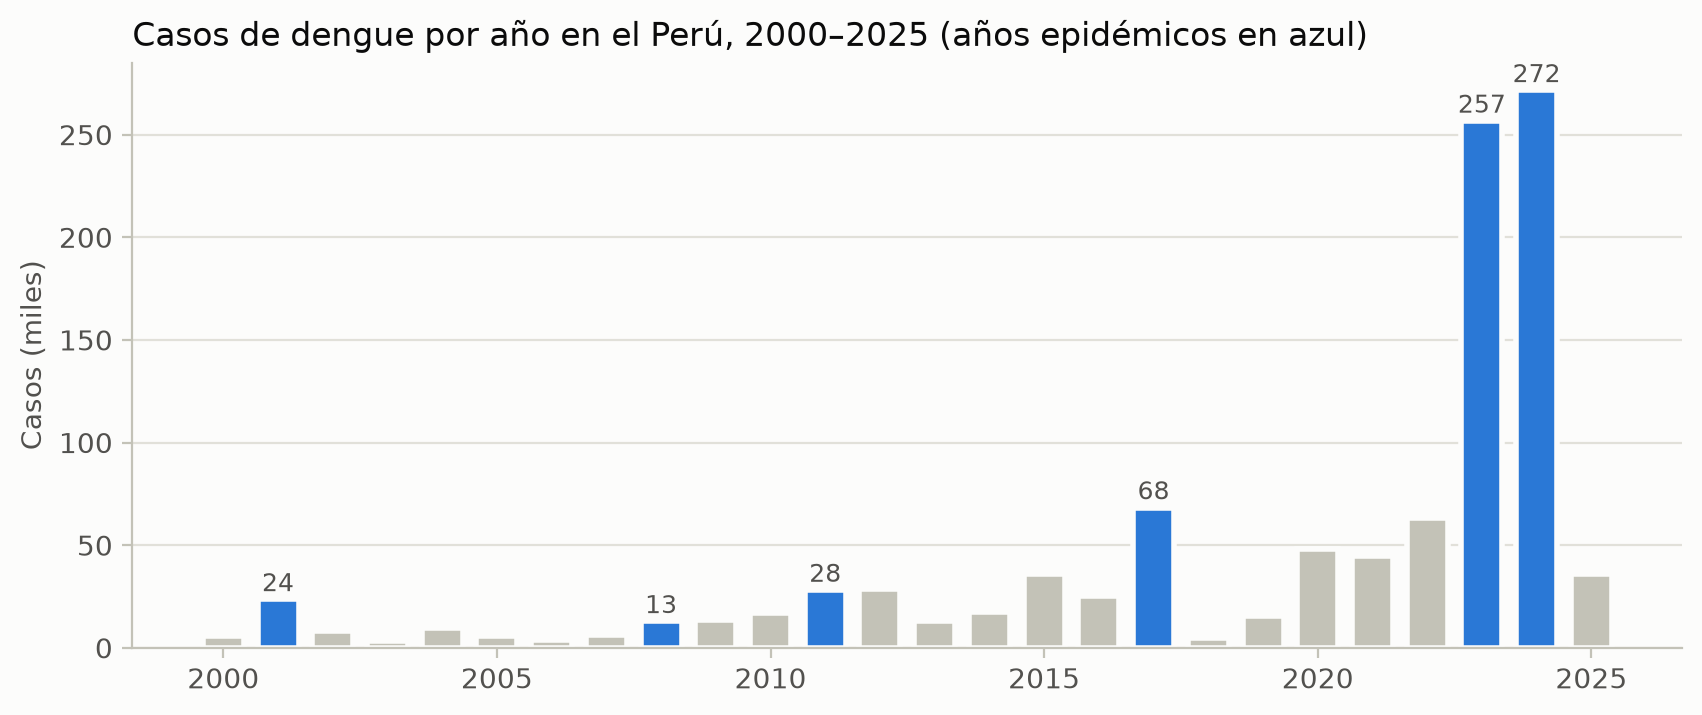
\includegraphics[width=0.72\textwidth]{q1_cases_per_year}
\caption{Casos de dengue por año, 2000–2025. En azul, los años epidémicos.}
\label{fig:q1}
\end{figure}

\paragraph{Q2 · Mayor incidencia.} El distrito con mayor incidencia fue La Huaca (Paita, Piura): 4,228 casos por
100,000 habitantes al año, unas 4 de cada 100 personas (Figura~\ref{fig:q2}). Se excluyeron los distritos con
menos de 10,000 habitantes, donde pocos casos producen tasas extremas. 10 de los 15 distritos con más incidencia
están en la costa, sobre todo en Piura y Áncash.

\begin{figure}[!htbp]
\centering
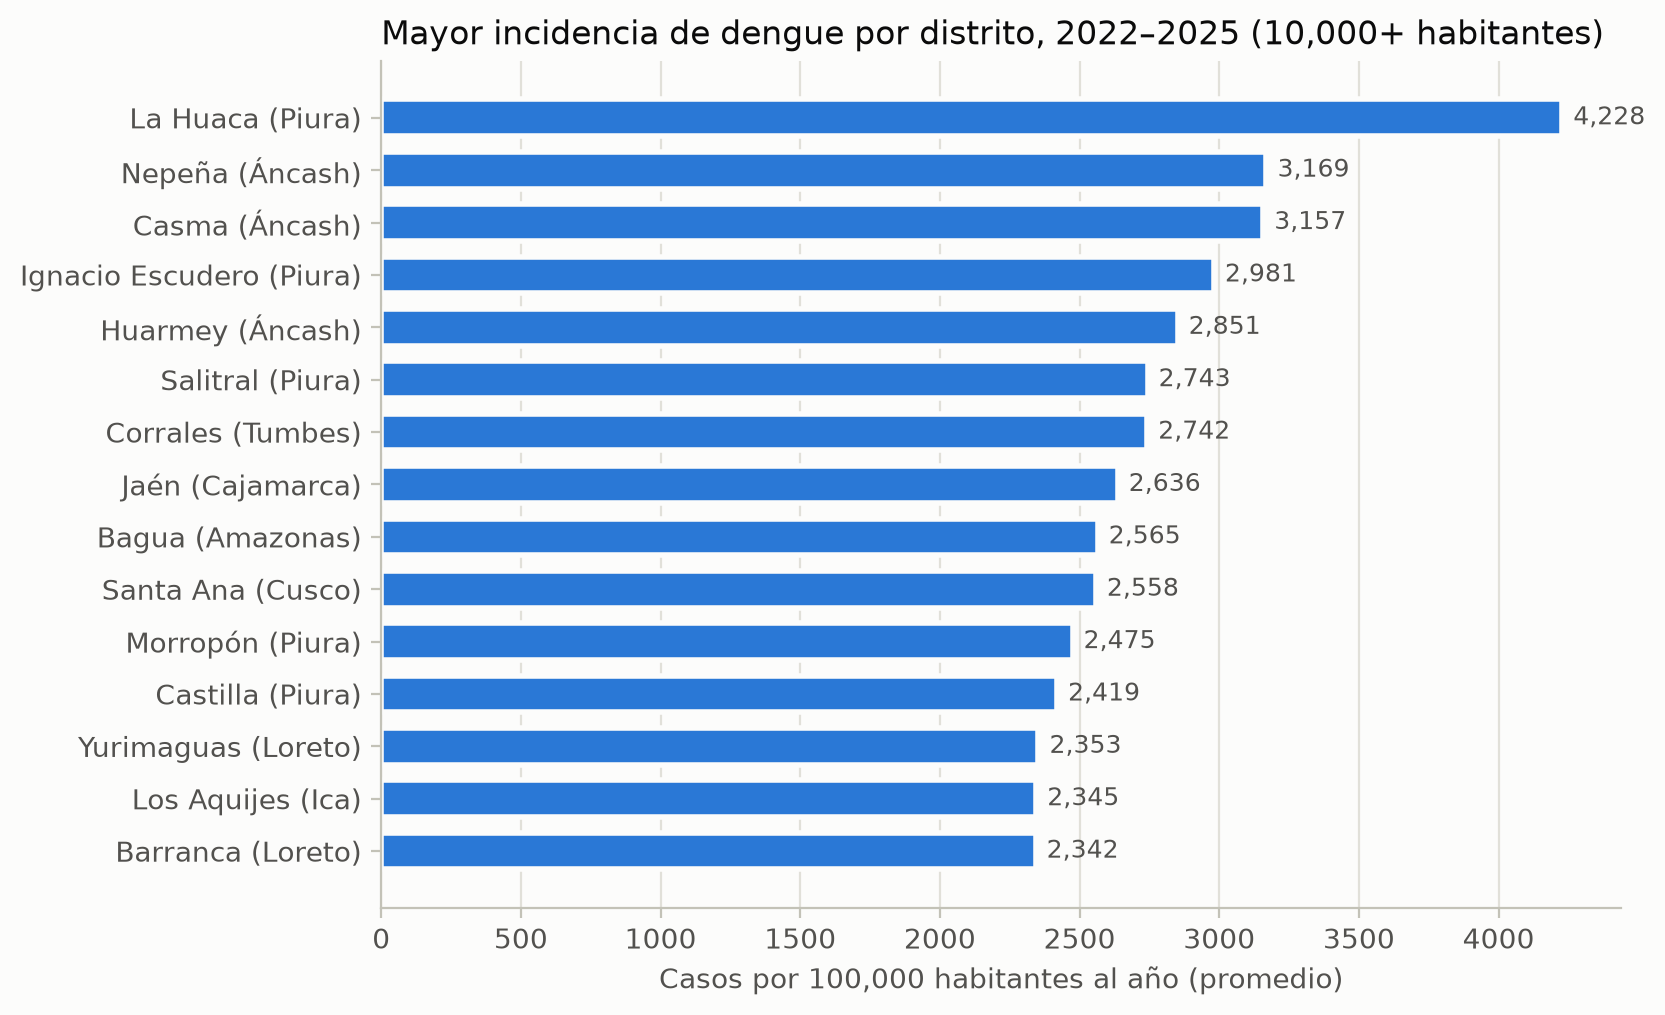
\includegraphics[width=0.5\textwidth]{q2_top_districts}
\caption{Los 15 distritos con mayor incidencia promedio, 2022–2025 (10,000 habitantes o más).}
\label{fig:q2}
\end{figure}

\paragraph{Q3 · Edad y sexo.} La incidencia más alta está en los adolescentes de 12 a 17 años, y las mujeres
superan a los hombres (479 frente a 405 casos por 100,000 al año) por las mujeres adultas
(Figura~\ref{fig:q3}). Los adultos de 30 a 59 años tienen más casos que cualquier otro grupo, pero solo porque es
el grupo con más población: por persona, su riesgo es igual al promedio nacional.

\paragraph{Q4 · Gravedad y establecimientos.} No hay relación. Los distritos con al menos 30 casos se dividieron
en cuatro grupos iguales según sus establecimientos activos por 10,000 habitantes (\code{ntile(4)}). La
proporción de casos con signos de alarma o graves es casi la misma en todos, entre 10\% y 13\%
(Figura~\ref{fig:q4}), y la correlación entre distritos es prácticamente nula ($r = 0.07$). La pequeña diferencia
va al revés de lo esperado: es algo mayor donde hay más establecimientos, probablemente porque ahí se detectan
mejor los signos de alarma.

\begin{figure}[!htbp]
\centering
\begin{subfigure}[b]{0.52\textwidth}
  \centering
  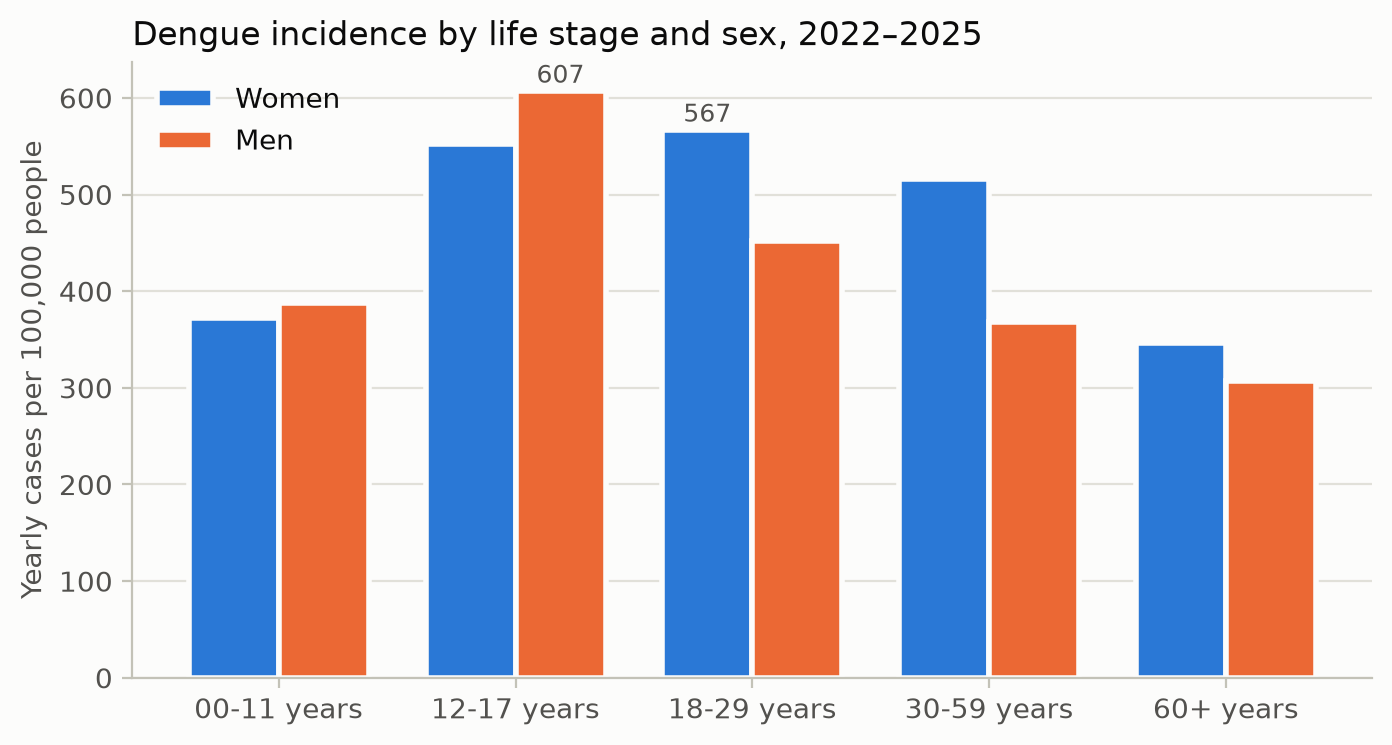
\includegraphics[width=\textwidth]{q3_age_sex}
  \caption{Q3: incidencia por etapa de vida y sexo.}
  \label{fig:q3}
\end{subfigure}\hfill
\begin{subfigure}[b]{0.46\textwidth}
  \centering
  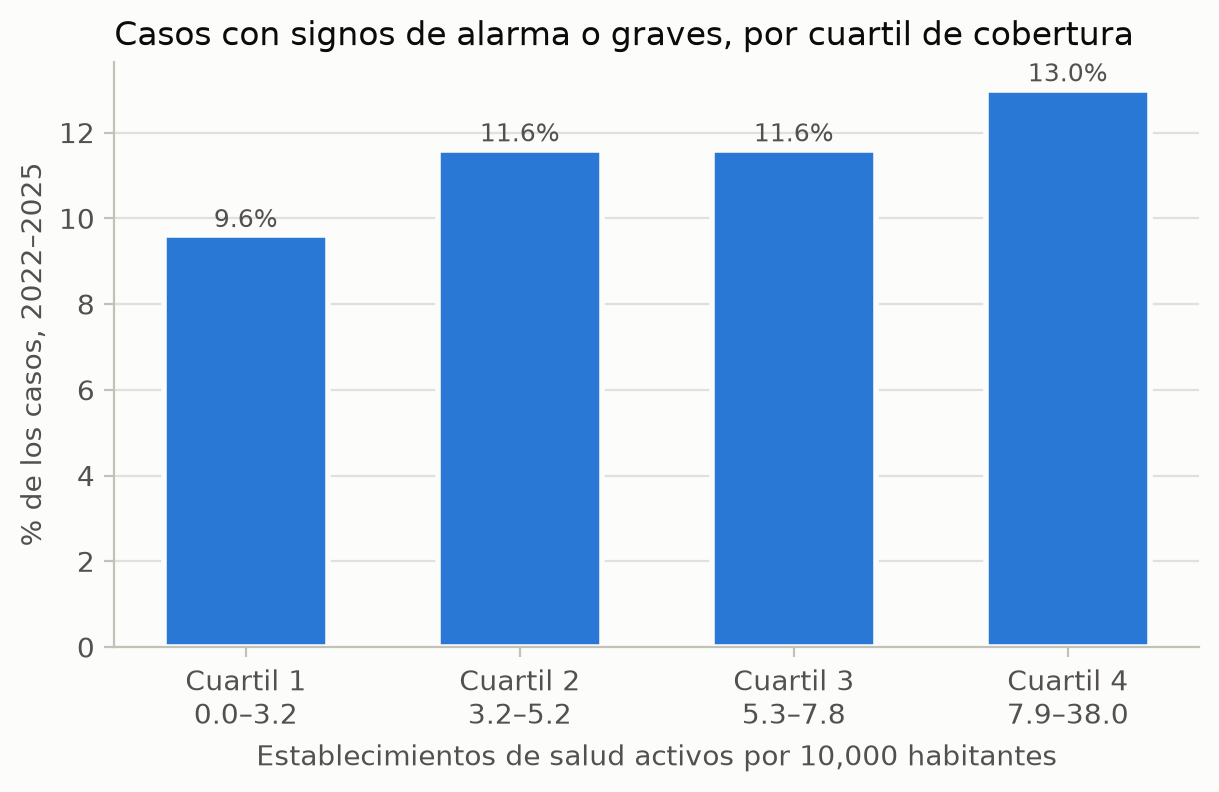
\includegraphics[width=\textwidth]{q4_severity_coverage}
  \caption{Q4: casos con signos de alarma o graves.}
  \label{fig:q4}
\end{subfigure}
\caption{Incidencia por grupo de población (Q3) y gravedad según la cobertura de establecimientos (Q4).}
\end{figure}

\paragraph{Q5 · Emergencias hídricas.} Sí, en las emergencias por lluvias. En los departamentos con al menos
1,000 casos en el año, los distritos en emergencia por lluvias tuvieron 2.3 veces más incidencia que los
distritos sin decreto en 2023, y 1.4 veces más en 2024 (Figura~\ref{fig:q5}). Las emergencias por déficit hídrico
no muestran ese aumento: se declararon sobre todo en departamentos andinos, donde casi no hay dengue. Entre los
distritos con decreto, los que tienen menos de 12 horas de agua al día tuvieron 3 veces más incidencia que los que
tienen entre 12 y 23 horas.

\begin{figure}[!htbp]
\centering
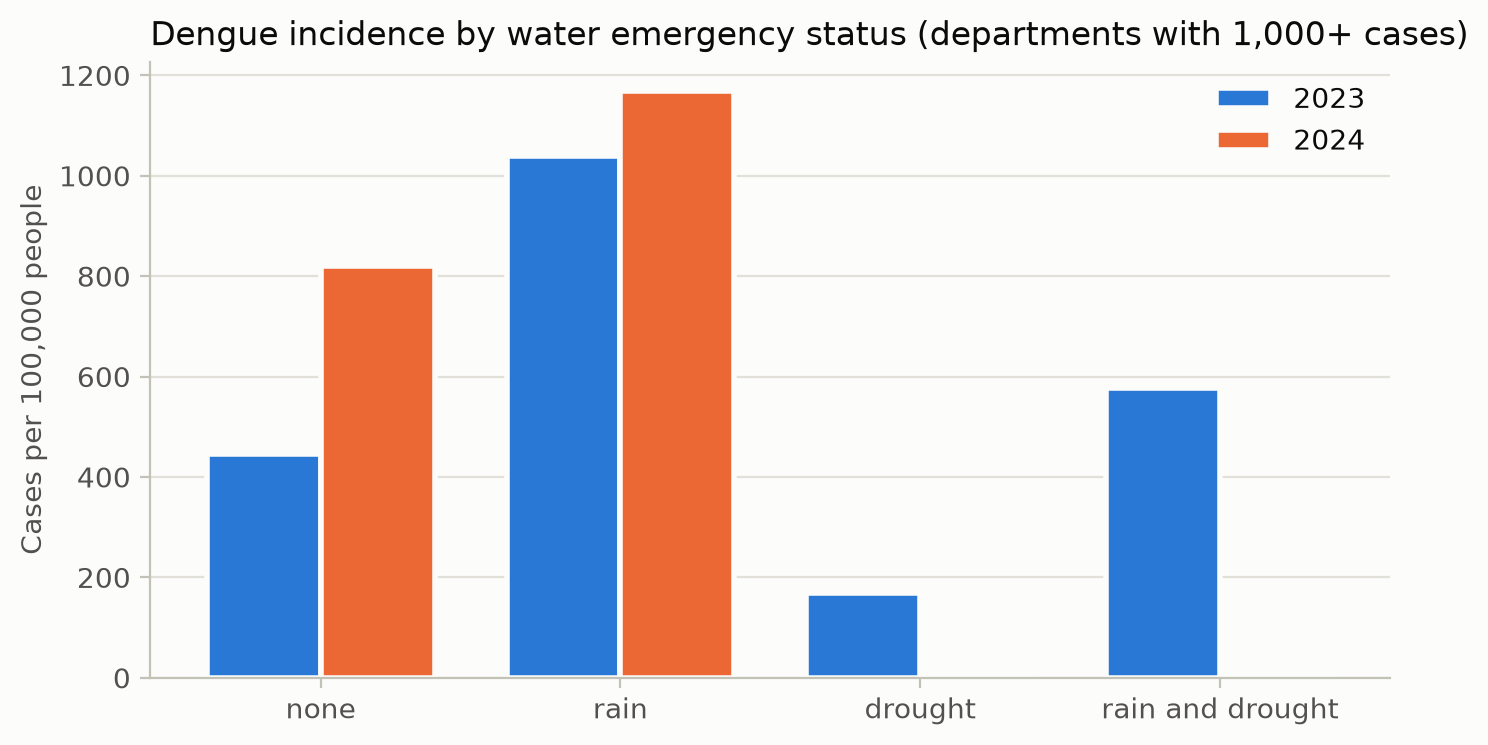
\includegraphics[width=0.5\textwidth]{q5_water_emergencies}
\caption{Incidencia según el tipo de emergencia hídrica del distrito, 2023 y 2024.}
\label{fig:q5}
\end{figure}

\paragraph{Q6 · Lluvia y casos.} Para cada estación se calculó la correlación entre la lluvia de la semana $t$ y
$\log(1 + \text{casos})$ de su provincia en la semana $t + k$, con $k$ de 0 a 12 semanas. El logaritmo evita que
las pocas semanas de pico, con miles de casos, decidan toda la correlación. En la costa, los casos aumentan entre
7 y 10 semanas después de la lluvia, con una relación moderada ($r$ de 0.26 a 0.44; Figura~\ref{fig:q6}): en
Piura, tras las lluvias de febrero a abril de 2023, los casos llegaron a su pico en mayo. En la selva no hay un
desfase claro ($r \le 0.26$): allí llueve todo el año, así que la lluvia no marca cuándo empieza un brote.

\begin{figure}[!htbp]
\centering
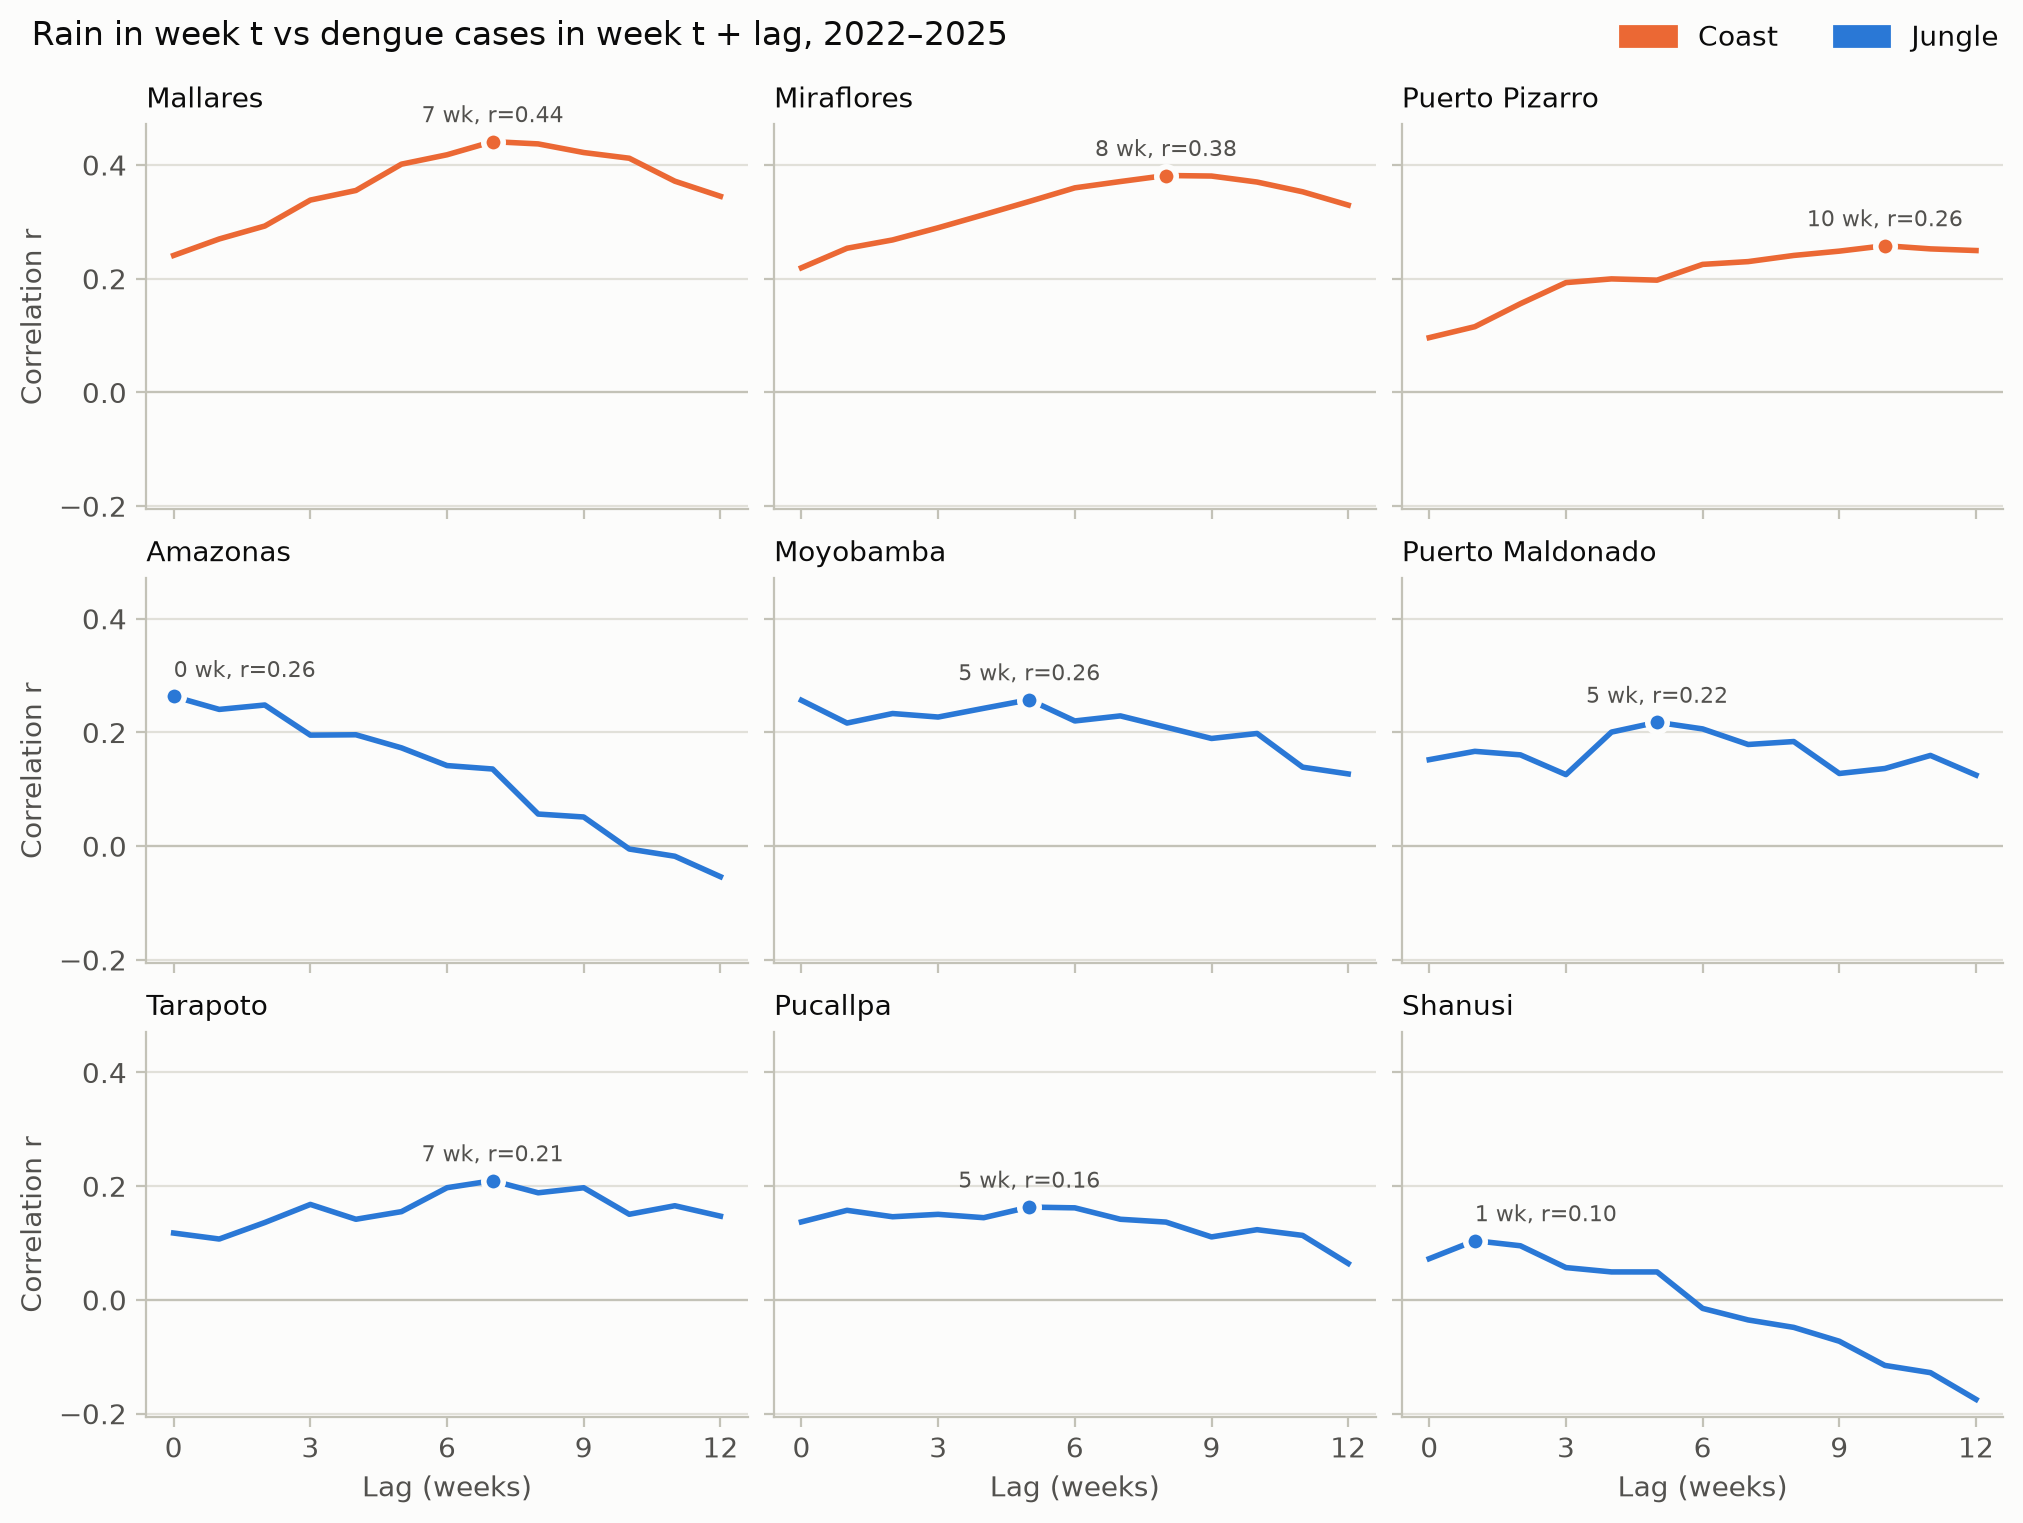
\includegraphics[width=0.56\textwidth]{q6_rain_lag_by_station}
\caption{Correlación entre la lluvia de la semana $t$ y los casos de la semana $t$ + desfase, por estación.}
\label{fig:q6}
\end{figure}

\paragraph{Limitaciones.} Los resultados son asociaciones, no relaciones causales. La población es la registrada
con DNI y no la censal; los establecimientos son un corte de 2026 frente a casos de 2022–2025; y las estaciones
tienen semanas sin datos, por lo que solo se usan las semanas con al menos 5 días medidos.

\section{Análisis de los planes de ejecución}
\label{sec:plans}

Spark no ejecuta las operaciones en el orden en que se escriben. Cada consulta pasa por varias fases
\cite{armbrust2015}: el analyzed logical plan (qué se pide, con nombres y tipos resueltos), el optimized logical
plan (las reglas de Catalyst lo reescriben), el physical plan (cómo se ejecuta cada operador) y, cuando llega una
action, la ejecución en stages y tasks. Esta sección analiza dos planes con \code{explain("formatted")}
(Figura~\ref{fig:plans}) y luego la ejecución completa de una consulta simple (notebook 03).

\begin{figure}[htbp]
\centering
\begin{minipage}[t]{0.585\textwidth}
\begin{lstlisting}[style=plan]
AdaptiveSparkPlan (25)
+- Sort (24)
   +- Exchange (23)
      +- Project (22)
         +- Filter (21)
            +- Window (20)
               +- WindowGroupLimit (19)
                  +- Sort (18)
                     +- Exchange (17)
                        +- WindowGroupLimit (16)
                           +- Sort (15)
                              +- Project (14)
                                 +- BroadcastHashJoin Inner BuildRight (13)
                                    :- HashAggregate (5)
                                    :  +- Exchange (4)
                                    :     +- HashAggregate (3)
                                    :        +- Filter (2)
                                    :           +- Scan parquet  (1)
                                    +- BroadcastExchange (12)
                                       +- Filter (11)
                                          +- HashAggregate (10)
                                             +- Exchange (9)
                                                +- HashAggregate (8)
                                                   +- Filter (7)
                                                      +- Scan parquet  (6)
\end{lstlisting}
\subcaption{Plan 1: top de distritos por incidencia (Q2).}
\label{fig:plan1}
\end{minipage}\hfill
\begin{minipage}[t]{0.385\textwidth}
\begin{lstlisting}[style=plan]
AdaptiveSparkPlan (9)
+- Project (8)
   +- BroadcastHashJoin LeftSemi BuildRight (7)
      :- Filter (2)
      :  +- Scan parquet  (1)
      +- BroadcastExchange (6)
         +- Project (5)
            +- Filter (4)
               +- Scan parquet  (3)
\end{lstlisting}
\subcaption{Plan 2: casos en distritos con emergencia por lluvias (Q5).}
\label{fig:plan2}
\end{minipage}
\caption{Physical plans de \code{explain("formatted")}. Solo se muestra el árbol; el número identifica a cada
operador en el detalle que imprime Spark.}
\label{fig:plans}
\end{figure}

\subsection{Plan 1: top de distritos por incidencia (Q2)}

\textbf{Logical plan.} Contar casos y sumar población por (año, distrito), unirlos con un left join, quedarse con
los distritos de 10,000 habitantes o más, calcular el ranking dentro de cada año y quedarse con el top 5.

\textbf{Optimización de Catalyst.}
\begin{enumerate}
  \item \textbf{Outer → inner join.} El filtro \code{population >= 10000} elimina las filas con nulos que
        agregaría el left join, así que Catalyst lo convierte en \code{Join Inner}.
  \item \textbf{Inferred filters y predicate pushdown.} El rango de años escrito solo para los casos llega
        también a la población a través del join key, y el filtro de población se aplica antes del join
        (operador 11).
  \item \textbf{Partition pruning.} \code{PartitionFilters: [year >= 2022, year <= 2025]}: solo se leen 4 de
        las 26 carpetas de años. El dynamic partition pruning agrega, en tiempo de ejecución, los años presentes
        en la población.
  \item \textbf{Column pruning.} El scan de casos lee \code{struct<ubigeo:string>}, 1 de 14 columnas (el año
        sale del nombre de la carpeta).
  \item \textbf{Top-N antes del shuffle.} \code{WindowGroupLimit} conserva los 5 mejores distritos por año antes
        del shuffle del window (16) y después (19).
\end{enumerate}

\textbf{Physical plan.} Cada agregación se hace en dos fases: un \code{HashAggregate} parcial en cada task, un
\code{Exchange} con \code{hashpartitioning} y un \code{HashAggregate} final (operadores 3–5 y 8–10). La población
agregada ocupa menos que el umbral de 10~MB de \code{autoBroadcastJoinThreshold}, así que se copia a cada task
(\code{BroadcastHashJoin Inner BuildRight}) y los casos no pasan por un shuffle para el join
\cite{spark-tuning}. El window necesita otro \code{Exchange} por \code{year} (17) y el \code{orderBy} final, un
\code{rangepartitioning} (23): en total, cuatro shuffles y un broadcast.

La versión en Spark SQL produce el mismo optimized logical plan y el mismo physical plan. Solo difieren el
parsed y el analyzed logical plan, porque el texto SQL se convierte en un árbol con CTEs: a Catalyst no le
importa con qué API se escribió la consulta.

\subsection{Plan 2: casos en distritos con emergencia por lluvias (Q5)}

\textbf{Logical plan.} Casos de 2023–2024 \code{left\_semi} join decretos por lluvias de 2023–2024, por
(año, distrito).

\textbf{Optimización de Catalyst.} Partition pruning (\code{year IN (2023, 2024)}: 2 de 26 carpetas), filter
pushdown al Parquet reader (\code{EqualTo(emergency\_type, rain)}, que permite saltar los row groups que no
pueden coincidir), column pruning (los casos leen solo \code{ubigeo}) y dynamic partition pruning.

\textbf{Physical plan: sin shuffle.} Los decretos filtrados son pocos, así que Spark hace broadcast de ellos como
una hash table (\code{BroadcastHashJoin LeftSemi BuildRight}). Cada task revisa sus propios casos contra esa
hash table y emite cada caso como máximo una vez, sin ningún \code{Exchange}. El inner join usa la misma
estrategia, pero emite una fila por cada decreto que coincide: 1,539,044 filas en lugar de 352,213.

\subsection{Lazy evaluation, DAG, stages y tasks}

Se usa la consulta de Q1: \code{cases.groupBy("year").agg(count).orderBy("year")}. Definirla tomó milisegundos y
no lanzó ningún job: \code{groupBy}, \code{agg} y \code{orderBy} son transformations que solo amplían el logical
plan. Recién el \code{collect()}, una action, hizo que Spark planificara y ejecutara la consulta.

La action convierte el physical plan en un DAG de stages, cortado en cada \code{Exchange}, porque un stage solo
puede empezar cuando sus datos de entrada ya fueron redistribuidos (Figura~\ref{fig:dag}). Cada stage se ejecuta
como tasks, una por partition: 9 para el scan (los archivos Parquet agrupados en 9 splits para 12 cores) y 1 en
los siguientes. Con AQE, cada stage con shuffle se lanza como su propio job, así que el \code{collect()} generó 4
jobs; los stages ya calculados aparecen como \emph{skipped} y reutilizan sus shuffle files. Dentro de un stage,
los operadores encadenados se compilan en una sola función Java (whole-stage code generation).

\begin{figure}[htbp]
\centering
\begin{tikzpicture}[
    stage/.style={draw=blue!60, fill=blue!8, rounded corners=2pt, align=center, font=\footnotesize,
                  text width=30mm, minimum height=13mm},
    arrow/.style={-{Stealth[length=2mm]}, thick, black!55},
    lbl/.style={font=\scriptsize, align=center, inner sep=1.5pt}]
  \node[stage] (s1) at (0, 0)       {\textbf{Stage 1 · 9 tasks}\\Scan parquet\\\code{partial\_count}};
  \node[stage] (s2) at (6.2, 1.1)   {\textbf{Stage 2 · 1 task}\\\code{count} final\\muestreo de sort keys};
  \node[stage] (s3) at (6.2, -1.1)  {\textbf{Stage 3 · 1 task}\\\code{count} final};
  \node[stage] (s4) at (12.4, -1.1) {\textbf{Stage 4 · 1 task}\\\code{Sort}\\26 filas al driver};
  \draw[arrow] (s1.east) -- (s2.west);
  \draw[arrow] (s1.east) -- (s3.west);
  \node[lbl] at (3.15, 0) {shuffle:\\\code{hashpartitioning}\\26 filas};
  \draw[arrow, dashed] (s2) -- node[lbl, right] {límites de\\los rangos} (s3);
  \draw[arrow] (s3) -- node[lbl, above] {shuffle:\\\code{rangepartitioning}} (s4);
\end{tikzpicture}
\caption{DAG de la consulta de Q1 con AQE: 4 stages, separados por los dos \code{Exchange} (shuffles).}
\label{fig:dag}
\end{figure}

\subsection{Shuffle}

Los casos de cada año están repartidos en archivos que leen tasks distintas. Para obtener un total por año, todos
los conteos parciales del mismo año deben llegar a la misma partition: \code{Exchange hashpartitioning(year)}
envía cada fila a la partition \code{hash(year) mod N}. Cada task escribe su salida en disco, agrupada por
partition de destino (\emph{shuffle write}), y las tasks del stage siguiente recogen su parte de cada una
(\emph{shuffle read}). Es el paso más costoso, porque implica disco, serialización y, en un cluster, red. El
\code{orderBy} necesita otro shuffle (\code{rangepartitioning}) para que cada partition tenga un rango de años.
La Tabla~\ref{tab:shuffle} compara la consulta con y sin adaptive query execution (AQE).

\begin{table}[htbp]
\centering
\caption{La consulta de Q1 con y sin AQE, según las métricas de la Spark UI.}
\label{tab:shuffle}
\small
\begin{tabular}{@{}lrr@{}}
\toprule
 & Con AQE & Sin AQE \\
\midrule
Tasks del scan & 9 & 9 \\
Filas leídas & 1,065,274 & 1,065,274 \\
Filas por shuffle (bytes) & 26 (1,664) & 26 (1,664) \\
Tasks después del shuffle & 1 + 1 + 1 & 200 + 200 + 26 \\
Tiempo del \code{collect()} & 0.14 s & 0.24 s \\
\bottomrule
\end{tabular}
\end{table}

La agregación parcial reduce el shuffle a 26 filas, una por año, en lugar de 1,065,274. Sin AQE, Spark usa las
200 partitions por defecto: 200 tasks procesan 26 filas, dos veces, más 26 tasks para el sort, casi todas vacías.
Con AQE, Spark mide el shuffle y lo reduce con coalesce a 1 partition \cite{spark-tuning}. Evitar shuffles es la
principal palanca de rendimiento: el plan 1 necesita cuatro, pero ninguno para su join gracias al broadcast, y el
plan 2 no necesita ninguno.

\section{Conclusiones}
\label{sec:conclusions}

\begin{itemize}
  \item El dengue en el Perú crece por brotes cada vez más grandes y se concentra en la costa norte y la selva.
        Los distritos en emergencia por lluvias y con menos horas de agua al día tuvieron más incidencia, y en la
        costa los casos aumentan unos dos meses después de la lluvia. No se encontró relación entre la gravedad
        de los casos y la cobertura de establecimientos de salud.
  \item Sobre la pregunta central: Spark convierte las operaciones en un logical plan; Catalyst lo optimiza
        (pruning, pushdown, joins reescritos); el physical plan decide cómo ejecutar cada operador; y una action
        lo divide en stages en cada shuffle y ejecuta cada stage como tasks en paralelo.
  \item La API no cambia la ejecución: la misma consulta en DataFrame API y en Spark SQL llega al mismo plan.
  \item El diseño de los datos se refleja en el plan: el particionado por año y el formato Parquet reducen lo que
        se lee, y el broadcast de las tablas pequeñas evita shuffles.
  \item El tipo de join define el resultado, no solo el costo: con filas repetidas, un inner join multiplicó los
        casos, mientras que un left semi join los contó una sola vez.
\end{itemize}


\printbibliography[heading=bibnumbered,title={Referencias}]

\end{document}
